\documentclass[a4paper, openany]{memoir}

\usepackage[utf8]{inputenc}
\usepackage[T1]{fontenc} 
\usepackage[english]{babel}

\usepackage{fancyhdr}
\usepackage{float}

\usepackage{amsmath}
\usepackage{amsthm}
\usepackage{amssymb}
\usepackage{enumitem}
\usepackage{multicol}
\usepackage[bookmarksopen=true,bookmarksopenlevel=2]{hyperref}
\usepackage{tikz}
\usepackage{listings}
\usepackage{xcolor}
\usepackage{indentfirst}
% \usepackage{graphicx}

\pagestyle{fancy}
\fancyhf{}
\fancyhead[LE]{\leftmark}
\fancyhead[RO]{\rightmark}
\fancyhead[RE, LO]{Algorithmics I}
\fancyfoot[LE, RO]{\thepage}
\fancyfoot[RE, LO]{Pete Gautam}
\usetikzlibrary{shapes, positioning, automata}
\definecolor{codegreen}{rgb}{0,0.6,0}
\definecolor{codegray}{rgb}{0.5,0.5,0.5}
\definecolor{codepurple}{rgb}{0.58,0,0.82}
\definecolor{backcolour}{rgb}{0.95,0.95,0.92}

\lstdefinestyle{thestyle}{
    backgroundcolor=\color{backcolour},
    basicstyle=\ttfamily\footnotesize,
    keywordstyle=\color{red!80}\bfseries,
    ndkeywordstyle=\color{blue!80}\bfseries,
    identifierstyle=\color{black},
    commentstyle=\color{codegreen},
    stringstyle=\color{codepurple},
    breakatwhitespace=false,
    breaklines=true,
    captionpos=b,
    keepspaces=true,
    numberstyle=\tiny\color{codegray},
    numbers=left,
    numbersep=2pt,
    showspaces=false,
    showstringspaces=false,
    showtabs=false,          
    tabsize=2
}

\lstdefinelanguage{pseudocode}{ 
    keywords={new, return, this, null, if, in, while, else, for, get, set, class, and, or, not, pass},
    ndkeywords={int, bool, List, String, Node, Queue, Set, Program, void, true, false},
    sensitive=true,
    comment=[l]{//},
    morecomment=[s]{/*}{*/},
    morestring=[b]',
    morestring=[b]"
}

\lstdefinelanguage{TM}{ 
    keywords={changeto, move, goto, is, if, while, module, accept, reject, halt},
    ndkeywords={left, right, direction, value, module_name, tapehead, program, basic_statements, blank},
    sensitive=true,
    comment=[l]{//},
    morecomment=[s]{/*}{*/},
    morestring=[b]',
    morestring=[b]"
}

\lstdefinelanguage{counter}{ 
    keywords={if, goto, halt},
    ndkeywords={},
    sensitive=true,
    comment=[l]{//},
    morecomment=[s]{/*}{*/},
    morestring=[b]',
    morestring=[b]"
}

\lstset{style=thestyle}

\usetikzlibrary{shapes, positioning, automata}

\chapterstyle{thatcher}

\setcounter{chapter}{4}

\begin{document}

\chapter{Introduction to computability}
\section{Computation and Decidability}
A computer takes some input $x$, acts on the input as a black box, and returns an output $f(x)$. In this section, we consider what the black box can do. It is a function that maps an input to an output. 

Computability concerns which functions can be computed. It is a formal way of answering `what problems can be solved by a computer', or alternatively `what problems cannot be solved by a computer'.

To answer such questions, we require a formal definition, i.e. the definition of what a computer is. Alternatively, we ask what an algorithm is if we view a computer as a device that can execute an algorithm.

There are some problems that cannot be solved by a computer, even with unbounded time. For example, consider the tiling problem. A tile is a $1 \times 1$ square that is divided into 4 triangles by its diagonals, with each triangle given a colour. Moreover, each tile has a fixed orientation, i.e. we cannot rotate them. For example, a tile is:
\begin{figure}[H]
    \centering
    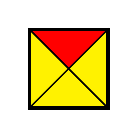
\begin{tikzpicture}
        \draw[fill=red] (0, 1) -- (1, 1) -- (.5, .5) -- cycle;
        \draw[fill=yellow] (0, 1) -- (0, 0) -- (.5, .5) -- cycle;
        \draw[fill=yellow] (0, 0) -- (1, 0) -- (.5, .5) -- cycle;
        \draw[fill=yellow] (1, 0) -- (1, 1) -- (.5, .5) -- cycle;
        
        \draw[very thick] (0, 0) rectangle (1, 1);
        \draw (0, 0) -- (1, 1)
            (1, 0) -- (0, 1);
    \end{tikzpicture}
\end{figure}
We now define the tiling problem.
\begin{itemize}
    \item \textbf{Name}: the tiling problem.
    \item \textbf{Instance}: a finite set $S$ of tile descriptions.
    \item \textbf{Question}: can any finite area, of any size, be completely covered using only tiles of types in $S$, so that adjacent tile colours match?
\end{itemize}
We illustrate this problem with an example. So, assume that we can use the following tiles.
\begin{figure}[H]
    \centering
    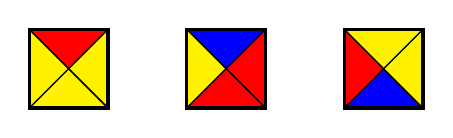
\begin{tikzpicture}
        \draw[fill=red] (0, 1) -- (1, 1) -- (.5, .5) -- cycle;
        \draw[fill=yellow] (0, 1) -- (0, 0) -- (.5, .5) -- cycle;
        \draw[fill=yellow] (0, 0) -- (1, 0) -- (.5, .5) -- cycle;
        \draw[fill=yellow] (1, 0) -- (1, 1) -- (.5, .5) -- cycle;
        
        \draw[very thick] (0, 0) rectangle (1, 1);
        \draw (0, 0) -- (1, 1)
            (1, 0) -- (0, 1);

        \draw[fill=blue] (2, 1) -- (3, 1) -- (2.5, .5) -- cycle;
        \draw[fill=yellow] (2, 1) -- (2, 0) -- (2.5, .5) -- cycle;
        \draw[fill=red] (2, 0) -- (3, 0) -- (2.5, .5) -- cycle;
        \draw[fill=red] (3, 0) -- (3, 1) -- (2.5, .5) -- cycle;
        
        \draw[very thick] (2, 0) rectangle (3, 1);
        \draw (2, 0) -- (3, 1)
            (3, 0) -- (2, 1);

        \draw[fill=yellow] (4, 1) -- (5, 1) -- (4.5, .5) -- cycle;
        \draw[fill=red] (4, 1) -- (4, 0) -- (4.5, .5) -- cycle;
        \draw[fill=blue] (4, 0) -- (5, 0) -- (4.5, .5) -- cycle;
        \draw[fill=yellow] (5, 0) -- (5, 1) -- (4.5, .5) -- cycle;
        
        \draw[very thick] (4, 0) rectangle (5, 1);
        \draw (4, 0) -- (5, 1)
            (5, 0) -- (4, 1);
    \end{tikzpicture}
    \caption{The available tiles.}
\end{figure}
\noindent Using these three tiles, we can make a $5 \times 5$ square as follows.
\begin{figure}[H]
    \centering
    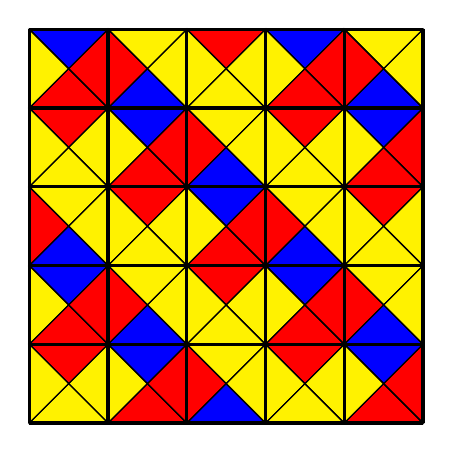
\begin{tikzpicture}
        \foreach \x/\y in {2/4, 0/3, 3/3, 1/2, 4/2, 2/1, 0/0, 3/0} {
            \draw[fill=red] (\x, \y+1) -- (\x+1, \y+1) -- (\x+.5, \y+.5) -- cycle;
            \draw[fill=yellow] (\x, \y+1) -- (\x, \y) -- (\x+.5, \y+.5) -- cycle;
            \draw[fill=yellow] (\x, \y) -- (\x+1, \y) -- (\x+.5, \y+.5) -- cycle;
            \draw[fill=yellow] (\x+1, \y) -- (\x+1, \y+1) -- (\x+.5, \y+.5) -- cycle;
        }
        
        \foreach \x/\y in {0/4, 3/4, 1/3, 4/3, 2/2, 0/1, 3/1, 1/0, 4/0} {
            \draw[fill=blue] (\x, \y+1) -- (\x+1, \y+1) -- (\x+.5, \y+.5) -- cycle;
            \draw[fill=yellow] (\x, \y+1) -- (\x, \y) -- (\x+.5, \y+.5) -- cycle;
            \draw[fill=red] (\x, \y) -- (\x+1, \y) -- (\x+.5, \y+.5) -- cycle;
            \draw[fill=red] (\x+1, \y) -- (\x+1, \y+1) -- (\x+.5, \y+.5) -- cycle;
        }
        
        \foreach \x/\y in {1/4, 4/4, 2/3, 0/2, 3/2, 1/1, 4/1, 2/0} {
            \draw[fill=yellow] (\x, \y+1) -- (\x+1, \y+1) -- (\x+.5, \y+.5) -- cycle;
            \draw[fill=red] (\x, \y+1) -- (\x, \y) -- (\x+.5, \y+.5) -- cycle;
            \draw[fill=blue] (\x, \y) -- (\x+1, \y) -- (\x+.5, \y+.5) -- cycle;
            \draw[fill=yellow] (\x+1, \y) -- (\x+1, \y+1) -- (\x+.5, \y+.5) -- cycle;
        }
        
        \draw[step=1, very thick] (0, 0) grid (5, 5);
        \draw (0, 0) -- (5, 5)
            (1, 0) -- (5, 4)
            (2, 0) -- (5, 3)
            (3, 0) -- (5, 2)
            (4, 0) -- (5, 1)
            (0, 1) -- (4, 5)
            (0, 2) -- (3, 5)
            (0, 3) -- (2, 5)
            (0, 4) -- (1, 5)
            
            (0, 5) -- (5, 0)
            (1, 5) -- (5, 1)
            (2, 5) -- (5, 2)
            (3, 5) -- (5, 3)
            (4, 5) -- (5, 4)
            (4, 0) -- (0, 4)
            (3, 0) -- (0, 3)
            (2, 0) -- (0, 2)
            (1, 0) -- (0, 1);
    \end{tikzpicture}
    \caption{A $5 \times 5$ square made using the tiles above.}
\end{figure}
\noindent We can further extend them to an $8 \times 5$ square, by adding the bottom 3 rows to the end of the $5 \times 5$ square, as shown below.
\begin{figure}[H]
    \centering
    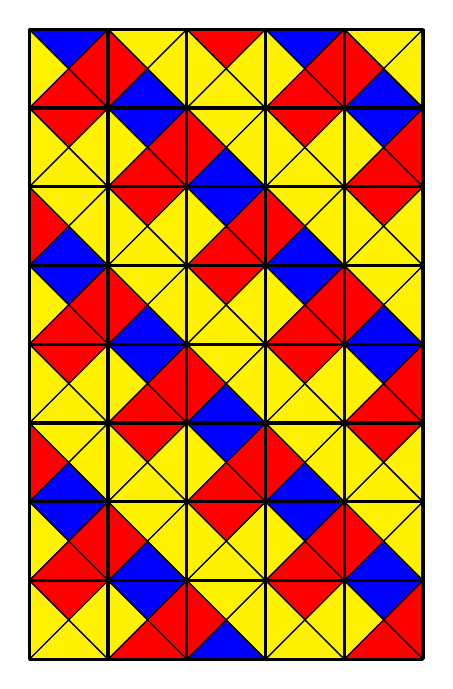
\begin{tikzpicture}
        \foreach \x/\y in {2/7, 0/6, 3/6, 1/5, 4/5, 2/4, 0/3, 3/3, 1/2, 4/2, 2/1, 0/0, 3/0} {
            \draw[fill=red] (\x, \y+1) -- (\x+1, \y+1) -- (\x+.5, \y+.5) -- cycle;
            \draw[fill=yellow] (\x, \y+1) -- (\x, \y) -- (\x+.5, \y+.5) -- cycle;
            \draw[fill=yellow] (\x, \y) -- (\x+1, \y) -- (\x+.5, \y+.5) -- cycle;
            \draw[fill=yellow] (\x+1, \y) -- (\x+1, \y+1) -- (\x+.5, \y+.5) -- cycle;
        }
        
        \foreach \x/\y in {0/7, 3/7, 1/6, 4/6, 2/5, 0/4, 3/4, 1/3, 4/3, 2/2, 0/1, 3/1, 1/0, 4/0} {
            \draw[fill=blue] (\x, \y+1) -- (\x+1, \y+1) -- (\x+.5, \y+.5) -- cycle;
            \draw[fill=yellow] (\x, \y+1) -- (\x, \y) -- (\x+.5, \y+.5) -- cycle;
            \draw[fill=red] (\x, \y) -- (\x+1, \y) -- (\x+.5, \y+.5) -- cycle;
            \draw[fill=red] (\x+1, \y) -- (\x+1, \y+1) -- (\x+.5, \y+.5) -- cycle;
        }
        
        \foreach \x/\y in {1/7, 4/7, 2/6, 0/5, 3/5, 1/4, 4/4, 2/3, 0/2, 3/2, 1/1, 4/1, 2/0} {
            \draw[fill=yellow] (\x, \y+1) -- (\x+1, \y+1) -- (\x+.5, \y+.5) -- cycle;
            \draw[fill=red] (\x, \y+1) -- (\x, \y) -- (\x+.5, \y+.5) -- cycle;
            \draw[fill=blue] (\x, \y) -- (\x+1, \y) -- (\x+.5, \y+.5) -- cycle;
            \draw[fill=yellow] (\x+1, \y) -- (\x+1, \y+1) -- (\x+.5, \y+.5) -- cycle;
        }
        
        \draw[step=1, very thick] (0, 0) grid (5, 8);
        \draw (0, 0) -- (5, 5)
            (1, 0) -- (5, 4)
            (2, 0) -- (5, 3)
            (3, 0) -- (5, 2)
            (4, 0) -- (5, 1)
            (0, 1) -- (5, 6)
            (0, 2) -- (5, 7)
            (0, 3) -- (5, 8)
            (0, 4) -- (4, 8)
            (0, 5) -- (3, 8)
            (0, 6) -- (2, 8)
            (0, 7) -- (1, 8)
            
            (0, 5) -- (5, 0)
            (0, 6) -- (5, 1)
            (0, 7) -- (5, 2)
            (0, 8) -- (5, 3)
            (1, 8) -- (5, 4)
            (2, 8) -- (5, 5)
            (3, 8) -- (5, 6)
            (4, 8) -- (5, 7)
            (4, 0) -- (0, 4)
            (3, 0) -- (0, 3)
            (2, 0) -- (0, 2)
            (1, 0) -- (0, 1);
    \end{tikzpicture}
    \caption{An $8 \times 5$ rectangle made using the tiles above.}
\end{figure}
\noindent In fact, we can keep adding the bottom 3 rows to the rectangle at the bottom. There is a similar way to extend it to the columns, meaning that these tiles can be used to tile any finite area.

Now, assume we have the following 3 tiles.
\begin{figure}[H]
    \centering
    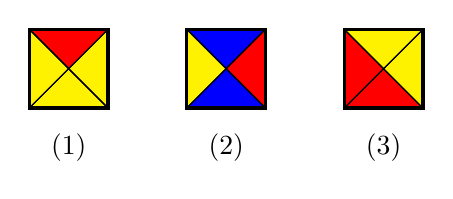
\begin{tikzpicture}
        \draw[fill=red] (0, 1) -- (1, 1) -- (.5, .5) -- cycle;
        \draw[fill=yellow] (0, 1) -- (0, 0) -- (.5, .5) -- cycle;
        \draw[fill=yellow] (0, 0) -- (1, 0) -- (.5, .5) -- cycle;
        \draw[fill=yellow] (1, 0) -- (1, 1) -- (.5, .5) -- cycle;
        
        \draw[very thick] (0, 0) rectangle (1, 1);
        \draw (0, 0) -- (1, 1)
            (1, 0) -- (0, 1);

        \draw[fill=blue] (2, 1) -- (3, 1) -- (2.5, .5) -- cycle;
        \draw[fill=yellow] (2, 1) -- (2, 0) -- (2.5, .5) -- cycle;
        \draw[fill=blue] (2, 0) -- (3, 0) -- (2.5, .5) -- cycle;
        \draw[fill=red] (3, 0) -- (3, 1) -- (2.5, .5) -- cycle;
        
        \draw[very thick] (2, 0) rectangle (3, 1);
        \draw (2, 0) -- (3, 1)
            (3, 0) -- (2, 1);

        \draw[fill=yellow] (4, 1) -- (5, 1) -- (4.5, .5) -- cycle;
        \draw[fill=red] (4, 1) -- (4, 0) -- (4.5, .5) -- cycle;
        \draw[fill=red] (4, 0) -- (5, 0) -- (4.5, .5) -- cycle;
        \draw[fill=yellow] (5, 0) -- (5, 1) -- (4.5, .5) -- cycle;
        
        \draw[very thick] (4, 0) rectangle (5, 1);
        \draw (4, 0) -- (5, 1)
            (5, 0) -- (4, 1);
        
        \foreach \x[count=\i] in {(1), (2), (3)} {
            \node at (2*\i-1.5, -0.5) {\x};
        }
    \end{tikzpicture}
\end{figure}
\noindent It is now impossible to tile a $3 \times 3$ square. We need to start from a tile that matches another tile in the right orientation, so we choose the tile (1) and stack tile (3) on top of it. We can only follow it with tile (1) at the top, and the first column is complete. Now, tile (1, 2) can be either tile (1) or tile (2)- we choose tile (2) first. In that case, the bottom two tiles in the second column must also be tile (2). Next, tile (2, 2) can only be tile (3). But then, we are stuck- there is no tile with top and bottom triangle red. Diagramatically, we are at the following state.
\begin{figure}[H]
    \centering
    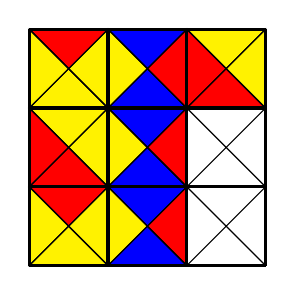
\begin{tikzpicture}
        \foreach \x/\y in {0/0, 0/2} {
            \draw[fill=red] (\x, \y+1) -- (\x+1, \y+1) -- (\x+.5, \y+.5) -- cycle;
            \draw[fill=yellow] (\x, \y+1) -- (\x, \y) -- (\x+.5, \y+.5) -- cycle;
            \draw[fill=yellow] (\x, \y) -- (\x+1, \y) -- (\x+.5, \y+.5) -- cycle;
            \draw[fill=yellow] (\x+1, \y) -- (\x+1, \y+1) -- (\x+.5, \y+.5) -- cycle;
        }
        
        \foreach \x/\y in {1/0, 1/1, 1/2} {
            \draw[fill=blue] (\x, \y+1) -- (\x+1, \y+1) -- (\x+.5, \y+.5) -- cycle;
            \draw[fill=yellow] (\x, \y+1) -- (\x, \y) -- (\x+.5, \y+.5) -- cycle;
            \draw[fill=blue] (\x, \y) -- (\x+1, \y) -- (\x+.5, \y+.5) -- cycle;
            \draw[fill=red] (\x+1, \y) -- (\x+1, \y+1) -- (\x+.5, \y+.5) -- cycle;
        }
        
        \foreach \x/\y in {0/1, 2/2} {
            \draw[fill=yellow] (\x, \y+1) -- (\x+1, \y+1) -- (\x+.5, \y+.5) -- cycle;
            \draw[fill=red] (\x, \y+1) -- (\x, \y) -- (\x+.5, \y+.5) -- cycle;
            \draw[fill=red] (\x, \y) -- (\x+1, \y) -- (\x+.5, \y+.5) -- cycle;
            \draw[fill=yellow] (\x+1, \y) -- (\x+1, \y+1) -- (\x+.5, \y+.5) -- cycle;
        }

        \draw[step=1, very thick] (0, 0) grid (3, 3);
        
        \draw (0, 0) -- (3, 3)
            (1, 0) -- (3, 2)
            (2, 0) -- (3, 1)
            (0, 1) -- (2, 3)
            (0, 2) -- (1, 3)
            
            (0, 3) -- (3, 0)
            (0, 2) -- (2, 0)
            (0, 1) -- (1, 0)
            (1, 3) -- (3, 1)
            (2, 3) -- (3, 2);
    \end{tikzpicture}
\end{figure}
\noindent We had a choice when choosing tile (1, 2). If we instead choose tile (1), then we are stuck already- the tile we need needs to have both top and left yellow. Diagrammatically, we are at the following state.
\begin{figure}[H]
    \centering
    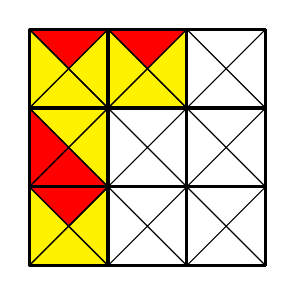
\begin{tikzpicture}
        \foreach \x/\y in {0/0, 0/2, 1/2} {
            \draw[fill=red] (\x, \y+1) -- (\x+1, \y+1) -- (\x+.5, \y+.5) -- cycle;
            \draw[fill=yellow] (\x, \y+1) -- (\x, \y) -- (\x+.5, \y+.5) -- cycle;
            \draw[fill=yellow] (\x, \y) -- (\x+1, \y) -- (\x+.5, \y+.5) -- cycle;
            \draw[fill=yellow] (\x+1, \y) -- (\x+1, \y+1) -- (\x+.5, \y+.5) -- cycle;
        }
        
        \foreach \x/\y in {} {
            \draw[fill=blue] (\x, \y+1) -- (\x+1, \y+1) -- (\x+.5, \y+.5) -- cycle;
            \draw[fill=yellow] (\x, \y+1) -- (\x, \y) -- (\x+.5, \y+.5) -- cycle;
            \draw[fill=blue] (\x, \y) -- (\x+1, \y) -- (\x+.5, \y+.5) -- cycle;
            \draw[fill=red] (\x+1, \y) -- (\x+1, \y+1) -- (\x+.5, \y+.5) -- cycle;
        }
        
        \foreach \x/\y in {0/1, } {
            \draw[fill=yellow] (\x, \y+1) -- (\x+1, \y+1) -- (\x+.5, \y+.5) -- cycle;
            \draw[fill=red] (\x, \y+1) -- (\x, \y) -- (\x+.5, \y+.5) -- cycle;
            \draw[fill=red] (\x, \y) -- (\x+1, \y) -- (\x+.5, \y+.5) -- cycle;
            \draw[fill=yellow] (\x+1, \y) -- (\x+1, \y+1) -- (\x+.5, \y+.5) -- cycle;
        }

        \draw[step=1, very thick] (0, 0) grid (3, 3);
        
        \draw (0, 0) -- (3, 3)
            (1, 0) -- (3, 2)
            (2, 0) -- (3, 1)
            (0, 1) -- (2, 3)
            (0, 2) -- (1, 3)
            
            (0, 3) -- (3, 0)
            (0, 2) -- (2, 0)
            (0, 1) -- (1, 0)
            (1, 3) -- (3, 1)
            (2, 3) -- (3, 2);
    \end{tikzpicture}
\end{figure}
\noindent So, the three tiles cannot be used to tile every finite area. 

In general, there is no algorithm that decides this problem. That is, if we have an algorithm $A$ that could solve this problem, then there are some tiles for which $A$ gives the wrong answer or $A$ does not terminate. The issue here is that we have to check all finite areas, and there are infinitely many of these. For certain sets of tiles that can tile any area, there is no repeated pattern like we saw in the first case. So, the algorithm would really have to check all finite areas for it to be correct- such an algorithm cannot terminate.

A problem $\Pi$ that admits no algorithm is called non-computable or unsolvable. If $\Pi$ is a decision problem and does not admit an algorithm, then it is called undecidable. The Tiling problem is undecidable.

Another undecidable problem is the post's correspondence problem (PCP).
\begin{itemize}
    \item \textbf{Name}: Post's correspondence Problem
    \item \textbf{Instance}: two finite sequences of words $X_1, \dots, X_n$ and $Y_1, \dots, Y_n$ over the same alphabet.
    \item \textbf{Question}: Does there exist a sequence $i_1, i_2, \dots, i_r$ of integers chosen from $\{1, \dots, n\}$ such that $X_{i_1} X_{i_2} \dots X_{i_r} = Y_{i_1} Y_{i_2} \dots Y_{i_r}$. That is, concatenating the $X_{ij}$'s and the $Y_{ij}$'s gives the same result.
\end{itemize}
For example, consider the case when $n = 5$ and we have the following sequence of words.
\begin{table}[H]
    \centering
    \begin{tabular}{cccc}
        \texttt{a} & \texttt{b} & \texttt{b} & \\
        \texttt{b} & \texttt{b} & \texttt{a} & \texttt{b}
    \end{tabular}
    \hspace{5pt}
    \begin{tabular}{cc}
        \texttt{a} & \\
        \texttt{a} & \texttt{a} 
    \end{tabular}
    \hspace{5pt}
    \begin{tabular}{ccc}
        \texttt{b} & \texttt{a} & \texttt{b} \\
        \texttt{a} & \texttt{b} 
    \end{tabular}
    \hspace{5pt}
    \begin{tabular}{cccc}
        \texttt{b} & \texttt{a} & \texttt{b} & \texttt{a} \\
        \texttt{a} & \texttt{a} 
    \end{tabular}
    \hspace{5pt}
    \begin{tabular}{ccc}
        \texttt{a} & \texttt{b} & \texttt{a} \\
        \texttt{a}
    \end{tabular}
\end{table}
\noindent Then, the sequence $2, 1, 1, 4, 1, 5$ gives the correspondence, as shown below.
\begin{figure}[H]
    \centering
    \begin{tabular}{ccccccccccccccccc}
        \texttt{\color{blue} a} & \texttt{\color{red} a} & \texttt{\color{red} b} & \texttt{\color{red} b} & \texttt{\color{blue} a} & \texttt{\color{blue} b} & \texttt{\color{blue} b} & \texttt{\color{red} b} & \texttt{\color{red} a} & \texttt{\color{red} b} & \texttt{\color{red} a} & \texttt{\color{blue} a} & \texttt{\color{blue} b} & \texttt{\color{blue} b} & \texttt{\color{red} a} & \texttt{\color{red} b} & \texttt{\color{red} a}\\
        \texttt{\color{blue} a} & \texttt{\color{blue} a} & \texttt{\color{red} b} &  \texttt{\color{red} b} & \texttt{\color{red} a} & \texttt{\color{red} b} & \texttt{\color{blue} b} & \texttt{\color{blue} b} & \texttt{\color{blue} a} & \texttt{\color{blue} b} & \texttt{\color{red} a} & \texttt{\color{red} a} & \texttt{\color{blue} b} & \texttt{\color{blue} b} & \texttt{\color{blue} a} & \texttt{\color{blue} b} & \texttt{\color{red} a}
    \end{tabular}
\end{figure}
Now, assume we have the following sequence of words.
\begin{table}[H]
    \centering
    \begin{tabular}{ccc}
        \texttt{b} & \texttt{b} & \\
        \texttt{b} & \texttt{a} & \texttt{b}
    \end{tabular}
    \hspace{5pt}
    \begin{tabular}{cc}
        \texttt{a} & \\
        \texttt{a} & \texttt{a} 
    \end{tabular}
    \hspace{5pt}
    \begin{tabular}{ccc}
        \texttt{b} & \texttt{a} & \texttt{b} \\
        \texttt{a} & \texttt{b} 
    \end{tabular}
    \hspace{5pt}
    \begin{tabular}{cccc}
        \texttt{b} & \texttt{a} & \texttt{b} & \texttt{a} \\
        \texttt{a} & \texttt{a} 
    \end{tabular}
    \hspace{5pt}
    \begin{tabular}{ccc}
        \texttt{a} & \texttt{b} & \texttt{a} \\
        \texttt{a}
    \end{tabular}
\end{table}
\noindent Then, there is no way to satisfy the correspondence condition. We can start with word (2) or (5) since the others would lead to a mismatch. If we start with (2), then we can only follow it with (2)- using (5) would lead to the \texttt{b} mismatching with an \texttt{a}. We can only continue on with (2), so we end up in a situation like this.
\begin{figure}[H]
    \centering
    \begin{tabular}{ccccccccccccccccc}
        \texttt{\color{blue} a} & \texttt{\color{red} a} & \texttt{\color{blue} a} \\
        \texttt{\color{blue} a} & \texttt{\color{blue} a} & \texttt{\color{red} a} & \texttt{\color{red} a} & \texttt{\color{blue} a} & \texttt{\color{blue} a}
    \end{tabular}
\end{figure}
\noindent There is no way that the two strings will match, so this will not work.

Instead, if we started with word (5), then we can only follow it with word (1). However, now we cannot use words (1), (3) or (4) since \texttt{b} and \texttt{a} would mismatch. So, we are stuck in the following state.
\begin{figure}[H]
    \centering
    \begin{tabular}{ccccccccccccccccc}
        \texttt{\color{blue} a} & \texttt{\color{blue} b} & \texttt{\color{blue} a} & \texttt{\color{red} b} & \texttt{\color{red} b} \\
        \texttt{\color{blue} a} & \texttt{\color{red} b} & \texttt{\color{red} a} & \texttt{\color{red} b}
    \end{tabular}
\end{figure}
\noindent So, there is no way to satisfy the correspondence condition with these 5 strings. It turns out that the PCP is also undecidable.

Next, we consider the halting problem.
\begin{itemize}
    \item \textbf{Name}: The Halting Problem (HP)
    \item \textbf{Instance}: A program $X$ and an input $S$.
    \item \textbf{Question}: Does the program $X$ halt on $S$?
\end{itemize}
That is, the algorithm returns \texttt{true} if $X$ halts when run on $S$, and instead returns \texttt{false} if $X$ enters an infinite loop when run with input $S$. We will prove that there cannot be an algorithm that decides the Halting problem.

First, consider the following program.
\lstinputlisting[language=pseudocode]{src/halting1.psc}
Clearly, this program halts if and only if $n \neq 1$. Now, consider the following program.
\lstinputlisting[language=pseudocode]{src/halting2.psc}
If we call the program with $n = 7$, we get the sequence: $7, 22, 11, 34, 17, 52, 26$, $13, 40, 20, 10, 5, 16, 8, 4, 2, 1$. So, the program above halts for $n = 7$. In general, we do not know whether this program halts for all values of $n$.

We shall now prove that HP is undecidable. So, assume for a contradiction that HP is decidable. In that case, we have an algorithm \texttt{halting} that decides HP. Now, define the following function \texttt{opposite}:
\lstinputlisting[language=pseudocode]{src/haltingContradiction.psc}
Now, run the program \texttt{opposite} on the program \texttt{opposite} itself. If \texttt{opposite} halts when it is given itself, then \texttt{opposite} loops. On the other hand, if \texttt{opposite} does not halt when it runs on itself, then \texttt{opposite} halts. Both of these statements are contradictions, so the programs \texttt{halting} and \texttt{opposite} cannot exist. Therefore, HP is undecidable.

We can prove that a problem is undecidable by reduction. Suppose that we can reduce any instance $I$ of $\Pi_1$ into an instance $J$ of $\Pi_2$ such that $I$ has a yes-answer for $\Pi_1$ if and only if $J$ has yes-answer for $\Pi_2$. Note that this algorithm need not be constructed in polynomial time. Now, if $\Pi_1$ is undecidable and we can perform such a reduction, then $\Pi_2$ is undecidable. Suppose for a contradiction that $\Pi_2$ is decidable. Then, we can use the reduction to decide $\Pi_1$. We can take $I$, and convert it into an instance of $J$. Since $\Pi_2$ is decidable, we can solve the instance $J$. Therefore, the instance $I$. This works for any instance $I$. Since $\Pi_1$ is undecidable, this is a contradiction. So, $\Pi_2$ must be undecidable.
\newpage

\section{Finite State Automata}
We shall now look at different models of computation to give a mathematical representation of a computer. We will look at three classical models of computation, of increasing power. The models are described below.
\begin{itemize}
    \item Finite state automata (FSA) are simple machines with a fixed amount of memory. They have very limited problem-solving ability, but they are still useful. 
    \item Pushdown automata (PDA) are simple machines with an unlimited amou-nt of memory that behaves like a stack.
    \item Turing machines (TM) are simple machines with unlimited memory that can be used arbitrarily. They essentially have the same power as a typical computer.
\end{itemize}

Deterministic finite-state automata (DFA) are simple machines with limited memory that recognise input on a read-only tape. It either recognises/accepts an input (which is made of characters from an alphabet), or does not recognise it. A DFA is made up of a finite input alphabet $\Sigma$, a finite set of states $Q$, an initial/start state $q_0 \in Q$ and a set of accepting states $F \subseteq Q$, along with a transition relation $T \subseteq (Q \times \Sigma) \times Q$, where $((q, a), q') \in T$ means that at state $q$, if we read an $a$, we go to $q'$. After we read the input, the input is recognised if and only if we end up at an accepting state. Determinism means that if $((q, a_1), q_1), ((q, a_2), q_2) \in T$, then either $a_1 \neq a_2$ or $q_1 = q_2$. That is, for any state and action, there is at most one move- we do not have a choice. We expect there to be precisely one way to move.

An example of a DFA is given below.
\begin{figure}[H]
    \centering
    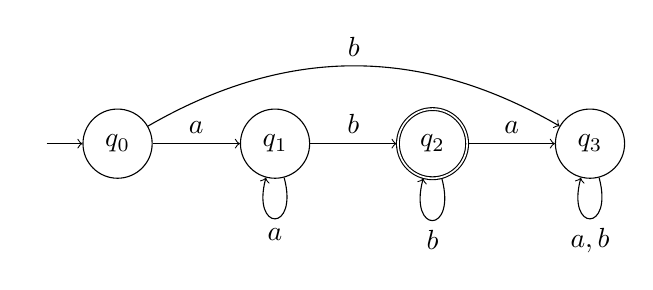
\begin{tikzpicture}
        \node[initial, state, initial text=] (q0) at (0, 0) {$q_0$};
        \node[state] (q1) at (2, 0) {$q_1$};
        \node[state, accepting] (q2) at (4, 0) {$q_2$};
        \node[state] (q3) at (6, 0) {$q_3$};
        
        \draw[->] (q0) to node[above] {$a$} (q1);
        \draw[->] (q1) to node[above] {$b$} (q2);
        \draw[->] (q2) to node[above] {$a$} (q3);
        \draw[->] (q1) to[loop below] node[below] {$a$} (q1);
        \draw[->] (q2) to[loop below] node[below] {$b$} (q2);
        \draw[->] (q3) to[loop below] node[below] {$a, b$} (q3);
        \draw[->] (q0) to[loop below, bend left] node[above] {$b$} (q3);
    \end{tikzpicture}
    \caption{A DFA}
\end{figure}
\noindent Here, the alphabet $\Sigma = \{a, b\}$, and the states $Q = \{q_0, q_1, q_2, q_3\}$, the initial state is $q_0$ (marked by the entering arrow), and there is only one accepting state- $q_2$ (marked by a double circle). The transition relation is shown by edges connecting the states, e.g. $((q_0, a), q_1) \in T$. This DFA recognises the strings $ab$ and $aaabb$, but it does not recognise $aabba$.

A DFA defines a language. Here, a language refers to a set of strings over some alphabet $\Sigma$. It determines whether the string on the input tape belongs to that language. In other words, it solves a decision problem. In the case above, we find that $ab$ and $aaabb$ belong to that language, but $aabba$ does not. In fact, the DFA recognises precisely the strings starting with an $a$, followed by as many $a$'s, and then a $b$, followed by as many $b$'s.

The following DFA recognises strings that contain two consecutive $a$'s.
\begin{figure}[H]
    \centering
    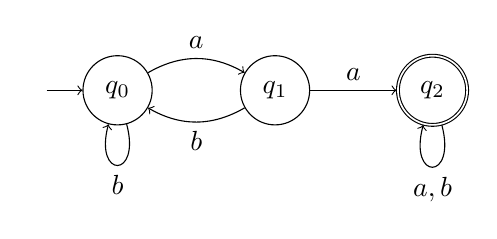
\begin{tikzpicture}
        \node[initial, state, initial text=] (q0) at (0, 0) {$q_0$};
        \node[state] (q1) at (2, 0) {$q_1$};
        \node[state, accepting] (q2) at (4, 0) {$q_2$};
        
        \draw[->] (q0) to[loop above, bend left] node[above] {$a$} (q1);
        \draw[->] (q1) to node[above] {$a$} (q2);
        \draw[->] (q0) to[loop below] node[below] {$b$} (q0);
        \draw[->] (q1) to[loop below, bend left] node[below] {$b$} (q0);
        \draw[->] (q2) to[loop below] node[below] {$a, b$} (q2);
    \end{tikzpicture}
    \caption{A DFA that recognises strings containing two consecutive $a$'s.}
\end{figure}
At the start, it is possible for the string to have as many $b$'s as possible (so, $((q_0, b), q_0) \in T$). As soon as we see 2 consecutive $a$, we're done- it doesn't matter what else we see (so, $((q_2, a), q_2), ((q_2, b), q_2) \in T$). If we see an $a$ then a $b$, we restart (so, $((q_1, b), q_0) \in T$).

The states in the DFA above have `memory'. In fact, we know that:
\begin{itemize}
    \item at state $q_0$, we know that the last character was a $b$;
    \item at state $q_1$, we know that the last character was an $a$, but the penultimate one was a $b$; and
    \item at state $q_2$, we know that we have seen two consecutive $a$'s before.
\end{itemize}
Although DFAs have some memory, it is very limited.

We can easily recognise the complement language, i.e. the set of strings that do not contain two consecutive $a$'s. We make an accepting state non-accepting, and a non-accepting state an accepting one. This is possible since the transition functions haven't changed, so the `memory' at each state remains the same as above. The DFA is shown below.
\begin{figure}[H]
    \centering
    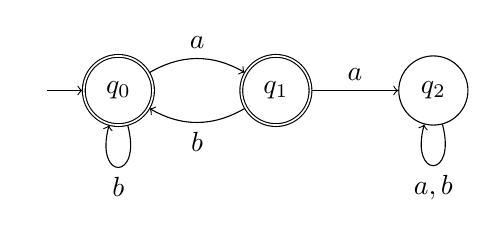
\begin{tikzpicture}
        \node[initial, state, initial text=, accepting] (q0) at (0, 0) {$q_0$};
        \node[state, accepting] (q1) at (2, 0) {$q_1$};
        \node[state] (q2) at (4, 0) {$q_2$};
        
        \draw[->] (q0) to[loop above, bend left] node[above] {$a$} (q1);
        \draw[->] (q1) to node[above] {$a$} (q2);
        \draw[->] (q0) to[loop below] node[below] {$b$} (q0);
        \draw[->] (q1) to[loop below, bend left] node[below] {$b$} (q0);
        \draw[->] (q2) to[loop below] node[below] {$a, b$} (q2);
    \end{tikzpicture}
    \caption{A DFA that recognises strings not containing two consecutive $a$'s.}
\end{figure}

The following FSA recognises strings that start and end with a $b$.
\begin{figure}[H]
    \centering
    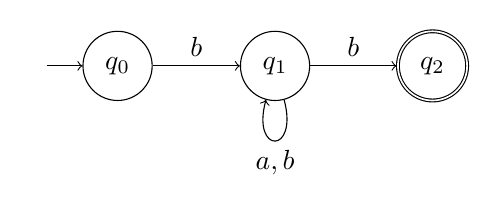
\begin{tikzpicture}
        \node[initial, state, initial text=] (q0) at (0, 0) {$q_0$};
        \node[state] (q1) at (2, 0) {$q_1$};
        \node[state, accepting] (q2) at (4, 0) {$q_2$};
        
        \draw[->] (q0) to node[above] {$b$} (q1);
        \draw[->] (q1) to node[above] {$b$} (q2);
        \draw[->] (q1) to[loop below] node[below] {$a, b$} (q1);
    \end{tikzpicture}
    \caption{An NFA that recognises strings that start and end with $b$.}
\end{figure}
\noindent However, it is not a DFA since $((q_1, b), q_1), ((q_1, b), q_2) \in T$- we have a choice when we see a $b$ in $q_1$- we can either stay at $q_1$ or go to $q_2$. This is a non-deterministic finite state automaton (NFA). We say that an NFA recognises a string if there is some way for the string to be accepted.

A DFA is an NFA by definition. However, every NFA can also be converted into a DFA. Therefore, non-determinism, in this case, does not expand the class of languages that can be recognised by a FSA.

We can reduce a NFA to a DFA using the subset construction. States of the DFA are sets of states of the NFA. So, construction can cause a blow-up in the number of states. In the worst case, we can go from $N$ states to $2^N$ states. However, typically not all sets of the states are required in the DFA. For example, in the case above, the following is the DFA corresponding to it.
\begin{figure}[H]
    \centering
    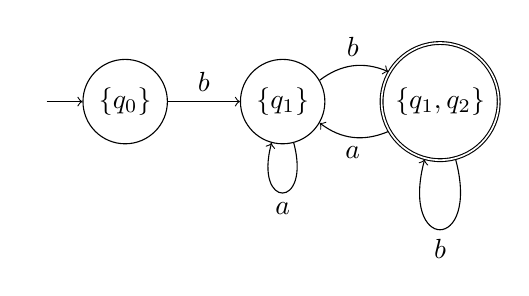
\begin{tikzpicture}
        \node[initial, state, initial text=] (q0) at (0, 0) {$\{q_0\}$};
        \node[state] (q1) at (2, 0) {$\{q_1\}$};
        \node[state, accepting] (q2) at (4, 0) {$\{q_1, q_2\}$};
        
        \draw[->] (q0) to node[above] {$b$} (q1);
        \draw[->] (q1) to[loop below, bend left] node[above] {$b$} (q2);
        \draw[->] (q1) to[loop below] node[below] {$a$} (q1);
        \draw[->] (q2) to[loop below] node[below] {$b$} (q2);
        \draw[->] (q2) to[loop below, bend left] node[below] {$a$} (q1);
    \end{tikzpicture}
    \caption{A DFA that recognises strings that start and end with $b$.}
\end{figure}
\noindent It only requires 3 states. Not all the possibilities are shown above- for example, we did not define what happens when we see an $a$ in the state $\{q_0\}$. This means that we automatically reject the string, i.e. a string starting with an $a$ is not part of this language.

The languages that can be recognised by DFAs are called the regular languages. A regular language (over an alphabet $\Sigma$) can be specified by a regular expression over $\Sigma$. Here,
\begin{itemize}
    \item The empty string $\epsilon$ is a regular expression;
    \item $\sigma$ is a regular expression for all characters $\sigma \in \Sigma$;
    \item If $R$ and $S$ are regular expressions, then their concatenation $RS$ is a regular expression;
    \item If $R$ and $S$ are regular expressions, then their union $R | S$ is also a regular expression;
    \item If $R$ is a regular expression, then its closure $R^*$ is a regular expression. $R^*$ denotes 0 or more copies of $R$;
    \item If $R$ is a regular expression, then $(R)$ is an regular expression as well. This is used to override precedence between operators.
\end{itemize}

The order of precedence is closure, then concatenation, then union. We can use brackets to override this order. So, suppose $\Sigma = \{a, b, c, d\}$. Then, $R = (ac | a^* b)d$ means $((ac) | ((a^*) b)) d$. The corresponding language is
\[\{acd, bd, abd, aabd, aaabd, \dots\}.\]

There are other operations as well, such as complement $\lnot x$, which is equivalent to the union of all characters in $\Sigma$ except $x$. We can also use $?$ to denote any character from $\Sigma$- it is equivalent to the union of all the characters.

We now formally define concatenation, union and closure. So, let $L(R)$ and $L(S)$ be the languages corresponding to the regular expression $R$ and $S$ respectively. Then, the concatenation is defined as
\[L(RS) = \{rs \mid r \in R, s \in S\}.\]
The union is defined as
\[L(R | S) = L(R) \cup L(S).\]
Finally, the closure is defined as
\[L(R^*) = L(R^0) \cup L(R^1) \cup L(R^2) \cup \cdots,\]
where $L(R^0) = \{\epsilon\}$ and $L(R^{i+1}) = L(RR^i)$. Importantly,
\[L(R^*) \neq \{r^* \mid r \in L(R)\}.\]
In fact, this language cannot be recognised by a DFA for certain regular expressions $R$. Essentially, for such a language, we would need a memory to remember which string in $r \in L(R)$ is repeated. Essentially, we would need at least one state for each element in $R$ to `remember' what pattern to repeat. However, $R$ might have infinite elements, and the number of states in a DFA must be finite. For example, if $R = a|b$, then the language of elementwise closure is given by $a^*|b^*$, which is regular. However, if $R = a(a|b)^*b$, then its elementwise closure is not regular.

Now, consider the language $(aa^* bb^*)^*$. This is the language composed of zero or more sequences which consist of a non-zero number of $a$'s followed by a non-zero number of $b$'s. The following DFA recognises the language.
\begin{figure}[H]
    \centering
    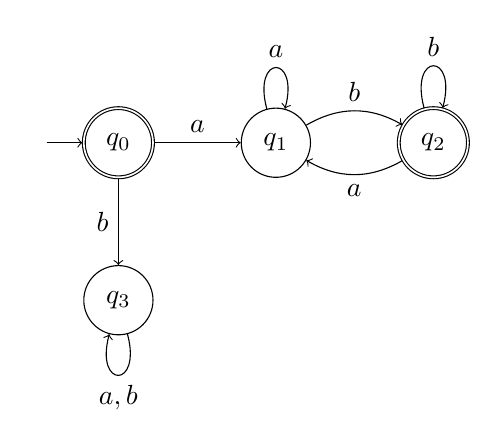
\begin{tikzpicture}
        \node[initial, state, accepting, initial text=] (q0) at (0, 0) {$q_0$};
        \node[state] (q1) at (2, 0) {$q_1$};
        \node[state, accepting] (q2) at (4, 0) {$q_2$};
        \node[state] (q3) at (0, -2) {$q_3$};
        
        \draw[->] (q0) to node[above] {$a$} (q1);
        \draw[->] (q0) to node[left] {$b$} (q3);
        \draw[->] (q3) to[loop below] node[below] {$a, b$} (q3);
        \draw[->] (q1) to[loop above] node[above] {$a$} (q1);
        \draw[->] (q2) to[loop below, bend left] node[below] {$a$} (q1);
        \draw[->] (q1) to[loop below, bend left] node[above] {$b$} (q2);
        \draw[->] (q2) to[loop above] node[above] {$b$} (q2);
    \end{tikzpicture}
    \caption{A DFA that recognises $(aa^*bb^*)^*$.}
\end{figure}
\noindent We accept the empty string, so $q_0$ is an accepting state. If we start with a $b$, then the string cannot be accepted- it `gets stuck' at $q_3$. If we start with an $a$, then we can have as many $a$'s after as we want, but the string can only get accepted if we see a $b$. After a $b$, if we see an $a$, then we can only accept the string if it is then followed by a $b$, and so on.

A DFA cannot recognise the language
\[L_1 = \{(a^m b^n)^* \mid m > 0, n > 0\}.\]
The problem is that the DFA would need to remember the values $m$ and $n$ to check that a string is in the language. But, there are infinitely many values for $m$ and $n$. Hence, a DFA would need to have an infinitely many states. This is not possible, so a DFA cannot recognise $L_1$. Similarly, a DFA cannot recognise
\[L_2 = \{a^n b^n \mid n > 0\}.\]
The languages that can be recognised by a DFA are called regular. The languages $L_1$ and $L_2$ are not regular.

Now, we look at some more DFAs. The DFA below recognises strings of the form $aa^*bb^*$.
\begin{figure}[H]
    \centering
    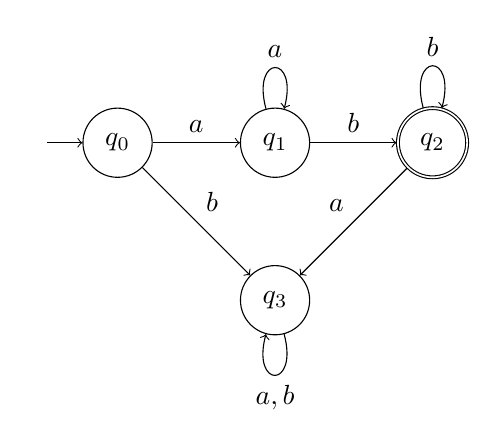
\begin{tikzpicture}
        \node[initial, state, initial text=] (q0) at (0, 0) {$q_0$};
        \node[state] (q1) at (2, 0) {$q_1$};
        \node[state, accepting] (q2) at (4, 0) {$q_2$};
        \node[state] (q3) at (2, -2) {$q_3$};
        
        \draw[->] (q0) to node[above] {$a$} (q1);
        \draw[->] (q1) to node[above] {$b$} (q2);
        \draw[->] (q2) to node[above left] {$a$} (q3);
        \draw[->] (q1) to[loop above] node[above] {$a$} (q1);
        \draw[->] (q2) to[loop above] node[above] {$b$} (q2);
        \draw[->] (q3) to[loop below] node[below] {$a, b$} (q3);
        \draw[->] (q0) to node[above right] {$b$} (q3);
    \end{tikzpicture}
    \caption{A DFA that recognises $aa^* bb^*$.}
\end{figure}
\noindent Moreover, the NFA below recognises $(a|b)^* aa (a|b)^*$- it has 2 consecutive $a$'s.
\begin{figure}[H]
    \centering
    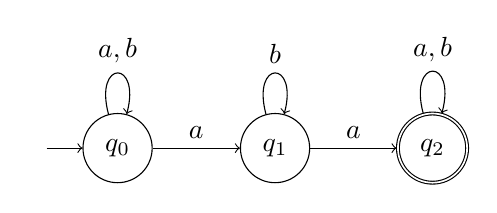
\begin{tikzpicture}
        \node[initial, state, initial text=] (q0) at (0, 0) {$q_0$};
        \node[state] (q1) at (2, 0) {$q_1$};
        \node[state, accepting] (q2) at (4, 0) {$q_2$};
        
        \draw[->] (q0) to node[above] {$a$} (q1);
        \draw[->] (q1) to node[above] {$a$} (q2);
        \draw[->] (q1) to[loop above] node[above] {$b$} (q1);
        \draw[->] (q0) to[loop above] node[above] {$a, b$} (q0);
        \draw[->] (q2) to[loop above] node[above] {$a, b$} (q2);
    \end{tikzpicture}
    \caption{An NFA that recognises $(a|b)^* aa (a|b)^*$.}
\end{figure}
\noindent The following DFA also recognises strings that contain consecutive $a$'s.
\begin{figure}[H]
    \centering
    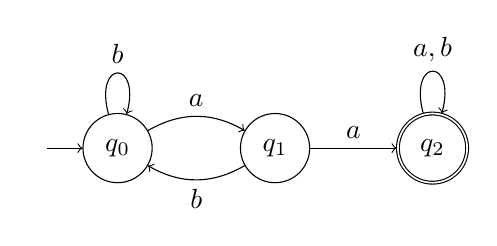
\begin{tikzpicture}
        \node[initial, state, initial text=] (q0) at (0, 0) {$q_0$};
        \node[state] (q1) at (2, 0) {$q_1$};
        \node[state, accepting] (q2) at (4, 0) {$q_2$};
        
        \draw[->] (q0) to[loop above] node[above] {$b$} (q0);
        \draw[->] (q0) to[loop above, bend left] node[above] {$a$} (q1);
        \draw[->] (q1) to[loop above, bend left] node[below] {$b$} (q0);
        \draw[->] (q1) to node[above] {$a$} (q2);
        % \draw[->] (q1) to[loop above] node[above] {$b$} (q1);
        \draw[->] (q2) to[loop above] node[above] {$a, b$} (q2);
    \end{tikzpicture}
    \caption{A DFA that recognises $(a|b)^* aa (a|b)^*$.}
\end{figure}
\noindent The following DFA recognises strings that do not contain consecutive $a$'s- the regular expression is $a|b^* (abb^*)^*$.
\begin{figure}[H]
    \centering
    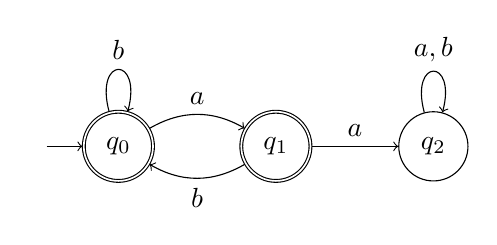
\begin{tikzpicture}
        \node[initial, state, initial text=, accepting] (q0) at (0, 0) {$q_0$};
        \node[state, accepting] (q1) at (2, 0) {$q_1$};
        \node[state] (q2) at (4, 0) {$q_2$};
        
        \draw[->] (q0) to[loop above] node[above] {$b$} (q0);
        \draw[->] (q0) to[loop above, bend left] node[above] {$a$} (q1);
        \draw[->] (q1) to[loop above, bend left] node[below] {$b$} (q0);
        \draw[->] (q1) to node[above] {$a$} (q2);
        \draw[->] (q2) to[loop above] node[above] {$a, b$} (q2);
    \end{tikzpicture}
    \caption{A DFA that recognises $a|b^* (abb^*)^*$.}
\end{figure}
% Two a's or b's => (a|b)*aa(a|b)*|(a|b)*bb(a|b)*
\noindent The following NFA recognises strings that start and end with a $b$.
\begin{figure}[H]
    \centering
    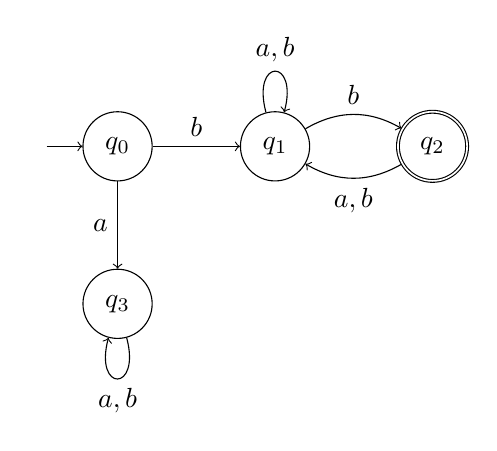
\begin{tikzpicture}
        \node[initial, state, initial text=] (q0) at (0, 0) {$q_0$};
        \node[state] (q1) at (2, 0) {$q_1$};
        \node[state, accepting] (q2) at (4, 0) {$q_2$};
        \node[state] (q3) at (0, -2) {$q_3$};
        
        \draw[->] (q0) to node[above] {$b$} (q1);
        \draw[->] (q1) to[loop above, bend left] node[above] {$b$} (q2);
        \draw[->] (q2) to[loop above, bend left] node[below] {$a, b$} (q1);
        \draw[->] (q0) to node[left] {$a$} (q3);
        \draw[->] (q3) to[loop below] node[below] {$a, b$} (q3);
        \draw[->] (q1) to[loop above] node[above] {$a, b$} (q1);        
    \end{tikzpicture}
    \caption{An NFA that recognises $b(a|b)^*b$.}
\end{figure}
\noindent The corresponding DFA for $b(a|b)^*b$ is given below.
\begin{figure}[H]
    \centering
    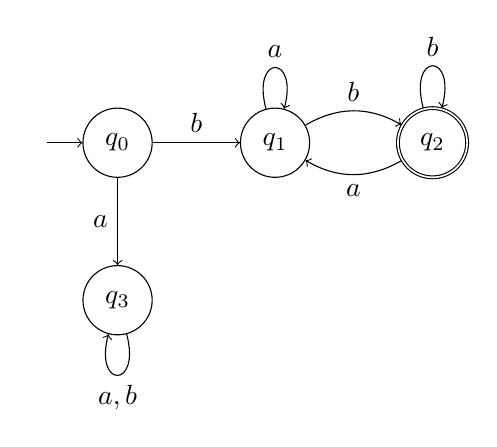
\begin{tikzpicture}
        \node[initial, state, initial text=] (q0) at (0, 0) {$q_0$};
        \node[state] (q1) at (2, 0) {$q_1$};
        \node[state, accepting] (q2) at (4, 0) {$q_2$};
        \node[state] (q3) at (0, -2) {$q_3$};
        
        \draw[->] (q0) to node[above] {$b$} (q1);
        \draw[->] (q1) to[loop above, bend left] node[above] {$b$} (q2);
        \draw[->] (q2) to[loop above, bend left] node[below] {$a$} (q1);
        \draw[->] (q0) to node[left] {$a$} (q3);
        \draw[->] (q3) to[loop below] node[below] {$a, b$} (q3);
        \draw[->] (q1) to[loop above] node[above] {$a$} (q1);        
        \draw[->] (q2) to[loop above] node[above] {$b$} (q2);
    \end{tikzpicture}
    \caption{A DFA that recognises $b(a|b)^*b$.}
\end{figure}
\noindent Finally, the following DFA recognises strings that contain an odd number of $a$'s- the regular expression is $b^* ab^*(ab^* ab^*)^*$.
\begin{figure}[H]
    \centering
    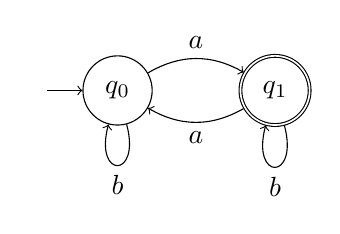
\begin{tikzpicture}
        \node[initial, state, initial text=] (q0) at (0, 0) {$q_0$};
        \node[state, accepting] (q1) at (2, 0) {$q_1$};
        
        \draw[->] (q0) to[loop above, bend left] node[above] {$a$} (q1);
        \draw[->] (q1) to[loop above, bend left] node[below] {$a$} (q0);
        \draw[->] (q0) to[loop below] node[below] {$b$} (q0);
        \draw[->] (q1) to[loop below] node[below] {$b$} (q1);
    \end{tikzpicture}
    \caption{A DFA that recognises $b^*a b^*(ab^*ab^*)^*$.}
\end{figure}
\newpage

\section{Pushdown Automata}
We saw that the language
\[L = \{a^n b^n \mid n > 0\}\]
cannot be recognised by a DFA. So, there are some functions/languages that we would regard as `computable' that cannot be computed by a finite-state automaton. Therefore, DFAs are not an adequate model of a general-purpose computer.

So, we consider another model of computation that recognises $L$. It cannot be done without extra memory, such as a stack. For instance, as we read $a$'s, we can push them onto a stack, and we can pop them as we read the $b$'s. The stack works as a counter and ensures that the number of $a$'s and $b$'s are equal.

Pushdown automata extend finite-state automata with a stack. It consists of a finite input alphabet $\Sigma$, a finite set of stack symbols $G$, a finite set of states $Q$, including a start state and a set of accepting states, and a control or transition relation $T \subseteq (Q \times \Sigma \cup \{\epsilon\} \times G \cup \{\epsilon\} \times (Q \times G \cup \{\epsilon\}))$, where $\epsilon$ is the empty string. A tuple $(q_a, w, \alpha, (q_b, \beta))$ represents a transition from the state $q_a$ to the state $q_b$ in the case where $w$ is the next letter on the input tape and $\alpha$ is on the top of the stack- this could then get popped and or we could push $\beta$. If we have the empty string $\epsilon$, then we do not pop and/or push. A PDA accepts an input if and only if after the input has been read, the stack is empty and the control is in an accepting state.

There is no explicit test to check that the stack is empty. However, this can be achieved by adding a special symbol (\$) to the stack at the start of the computation. We never add the symbol at any other point during the computation. Therefore, we can check that the stack is empty by checking whether the symbol \$ is on the top of the stack.

The PDAs defined here are non-deterministic. In this case, deterministic PDAs are less powerful. This differs from finite state automata where non-determinism does not add any power. So, there are languages that can be recognised by a non-deterministic PDA but not by a deterministic PDA. An example of this is the language of palindromes. A palindrome is a string that reads the same both forwards and backwards.

Using a PDA, we can recognise a palindrome by pushing the first half of the sequence onto the stack. Then, as we read each new character, we check if it is the same as the top element on the stack and we pop this element. We then enter an accepting state if all the checks succeed. Also, if the string is of odd length, then the middle character should not be added to the stack.

We require non-determinism here to know when to stop pushing onto the stack. We also need it since we do not know whether the length of the string is even or odd. We cannot work this out first and then check the string since we would need to read the string twice- this is not possible with a stack. We would need an unbounded number of states as the string could be of any finite length.

Now, we consider an example.
\begin{figure}[H]
    \centering
    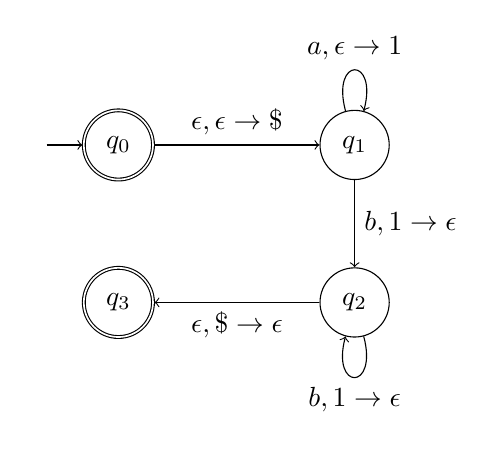
\begin{tikzpicture}
        \node[initial, state, initial text=, accepting] (q0) at (0, 0) {$q_0$};
        \node[state] (q1) at (3, 0) {$q_1$};
        \node[state] (q2) at (3, -2) {$q_2$};
        \node[state, accepting] (q3) at (0, -2) {$q_3$};
        
        \draw[->] (q0) to node[above] {$\epsilon, \epsilon \to \$$} (q1);
        \draw[->] (q1) to node[right] {$b, 1 \to \epsilon$} (q2);
        \draw[->] (q2) to node[below] {$\epsilon, \$ \to \epsilon$} (q3);
        \draw[->] (q1) to[loop above] node[above] {$a, \epsilon \to 1$} (q1);
        \draw[->] (q2) to[loop below] node[below] {$b, 1 \to \epsilon$} (q2);
    \end{tikzpicture}
\end{figure}
\noindent Here, we start at $q_0$. An empty string is accepted since $q_0$ is an accepting state. We first add \$ to the stack to mark the bottom of the stack. Next, if we encounter an $a$, we add 1 to the stack. Instead, if we encounter a $b$, we remove 1 from the stack. If we get to the end of the string with an empty stack (i.e. all the 1's have been removed), then we remove \$ and get to an accepting state. This PDA therefore recognises strings of the form $a^n b^n$ for $n \geq 0$. If there are more $a$'s than $b$'s, then the stack doesn't get emptied by the end of the string, and we are stuck at $q_2$. Instead, if there are more $b$'s than $a$'s, then we get stuck at $q_3$ with the input not completely read.

Clearly, PDAs are more powerful than FSMs. For example, the language
\[L = \{a^n b^n \mid n \geq 0\}\]
cannot be recognised by a FSM, but is recognised by a PDA. The languges that can be recognised by a non-deterministic PDA are called context-free languages. However, a PDA is not an adequate model of a general purpose computer. For example, it cannot recognise the language
\[L = \{a^n b^n c^n \mid n \geq 0\},\]
although we can write a program that recognises it.
\newpage

\section{Turing Machines}
A Turing machine is used to recognise a particular language, and consists of:
\begin{itemize}
    \item a finite alphabet $\Sigma$, including a blank symbol (denoted by \#);
    \item an unbound tape of squares, where each square can hold a single symbol of $\Sigma$, and the tape is unbounded in both directions;
    \item a tape head that scans a single square, which can read the square and write to it, and then move one square left or right;
    \item a set of states, including a starting state $s_0$ and two halting states- accepting $s_Y$ and rejecting $s_N$;
    \item a transition function, which tells us how to go from one state to other, what character to read from the tape, what to write to the tape and which way to move the tape head. It is of the form
    \[f: ((S \setminus \{s_Y, s_N\}) \times \Sigma) \to (S \times \Sigma \times \{\texttt{left}, \texttt{right}\}).\]
    If $f(s, \sigma) = (s', \sigma', d)$, then we read the symbol $\sigma$ from the tape in state $s$. We then move it to state $s'$, overwrite the symbol $\sigma$ on the tape with the symbol $\sigma'$, and move the tape head one square in the direction $d \in \{\texttt{left}, \texttt{right}\}$.
\end{itemize}
The (finite) input string is placed on the tape. We assume initially that all the other squares of the tape contain blanks. The tape head is placed on the first symbol of the input. The Turing machine starts in state $s_0$. If the machine halts in $s_Y$, the answer is \texttt{yes}- the input gets accepted. Instead, if the machine halts in $s_N$, the answer is \texttt{no}- the input gets rejected.

We now consider the palindrome problem. We can write a simple program in a high-level language to do this, as shown below.
\lstinputlisting[language=pseudocode]{src/palindrome.psc}
We will design a Turing machine that solves this problem. For simplicity, we assume that the string is composed of $a$'s and $b$'s. Formally defining a Turing machine for even simple problems is hard, so we will start with a pseudocode version. Turing machines are quite simple, making them easy to do proofs in. However, this simplicity also means that it is not easy to program using them. 

\newpage
The pseudocode that solves the palindrome problem for Turing machines is given below.
\lstinputlisting[language=TM]{src/palindromeTM.tm}

We need the following states, with the alphabet $\Sigma = \{\#, a, b\}$: $s_0$ to read and erase the leftmost symbol; $s_1, s_2$ to move right to look for the end, remembering the erased symbol, i.e. $s_1$ when read (and erased) $a$ and $s_2$ when read (and erased) $b$; $s_3, s_4$ to test for the appropriate rightmost symbol, i.e. $s_3$ testing against $a$ and $s_4$ testing against $b$; and $s_5$ to move back to the leftmost symbol.

Next, we consider the transition between the states. From $s_0$, we enter $s_Y$ if a blank is read, or move to $s_1$ or $s_2$ depending on whether an $a$ or a $b$ is read, erasing it in either case. We stay in $s_1$ or $s_2$, moving right until a blank is read, at which point, we enter $s_3$ or $s_4$, and move left. From $s_3$ or $s_4$, we enter $s_Y$ if a blank is read, $s_N$ if the `wrong' symbol is read. Otherwise, we erase it, and enter $s_5$, and move left. In $s_5$, we move left until a blank is read, then move right and enter $s_0$.

The Turing machine for the palindrome problem is therefore the following.
\begin{figure}[H]
    \centering
    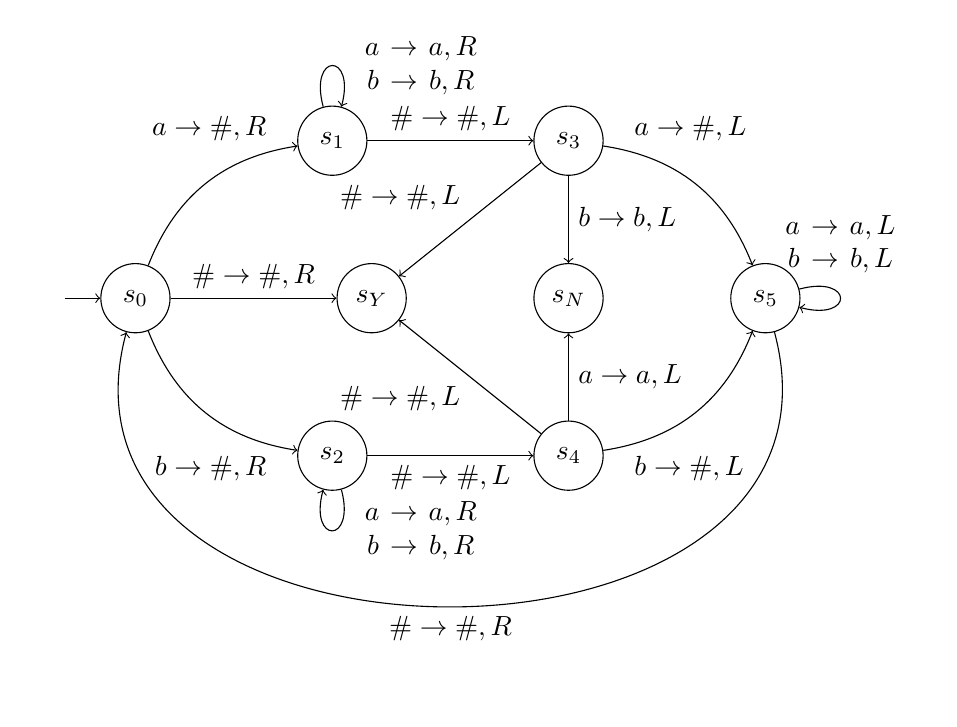
\begin{tikzpicture}
        \node[state, initial, initial text=] (s0) at (-.5, 0) {$s_0$};
        \node[state] (s1) at (2, 2) {$s_1$};
        \node[state] (s2) at (2, -2) {$s_2$};
        \node[state] (s3) at (5, 2) {$s_3$};
        \node[state] (s4) at (5, -2) {$s_4$};
        \node[state] (s5) at (7.5, 0) {$s_5$};
        \node[state] (sY) at (2.5, 0) {$s_Y$};
        \node[state] (sN) at (5, 0) {$s_N$};
        
        \draw[->] (s0) to[loop above, bend left] node[above left, pos=0.9] {$a \to \#, R$} (s1);
        \draw[->] (s1) to[loop above] node[right, text width=2cm, align=center] {$a \to a, R$ $b \to b, R$} (s2);
        \draw[->] (s1) to node[above] {$\# \to \#, L$} (s3);
        
        \draw[->] (s0) to[loop above, bend right] node[below left, pos=0.9] {$b \to \#, R$} (s2);
        \draw[->] (s2) to[loop below] node[right, text width=2cm, align=center] {$a \to a, R$ $b \to b, R$} (s2);
        \draw[->] (s2) to node[below] {$\# \to \#, L$} (s4);
        
        \draw[->] (s0) to node[above] {$\# \to \#, R$} (sY);
        \draw[->] (s3) to node[above left] {$\# \to \#, L$} (sY);
        \draw[->] (s4) to node[below left] {$\# \to \#, L$} (sY);
        
        \draw[->] (s4) to node[right] {$a \to a, L$} (sN);
        \draw[->] (s3) to node[right] {$b \to b, L$} (sN);
        
        \draw[->] (s3) to[loop below, bend left] node[above right, pos=0.1] {$a \to \#, L$} (s5);
        \draw[->] (s4) to[loop above, bend right] node[below right, pos=0.1] {$b \to \#, L$} (s5);
        
        \draw[->] (s5) to[loop right] node[above=2mm, text width=2cm, align=center] {$a \to a, L$ $b \to b, L$} (s5);
        \draw[->] (s5) to[loop below, looseness=1.5] node[below] {$\# \to \#, R$} (s0);
    \end{tikzpicture}
    \caption{A Turing machine that recognises palindromes over the alphabet $\Sigma = \{a, b\}$.}
\end{figure}

A Turing machine can be described by its state transition diagram, which is a directed graph where each state is represented by a vertex, and $f(s, \sigma) = (s', \sigma', d)$ is represented by an edge from vertex $s$ to vertex $s'$, labelled $\sigma \to \sigma', d$.

We shall now show that the language consisting of strings of the form $a^n b^m c^{n+m}$, for $n, m \geq 0$ is decidable. One solution is to first delete the $a$'s from the start each time and delete a corresponding $c$ from the end of the string. This will not introduce blanks as we are merely deleting from the start and the end. So, there is no ambiguity as to where the start and the end of the string is. After we have deleted all the $a$'s, we are left with $b^m c^m$, so we delete one $b$ from the front and one $c$ from the end. To do this, we need two `restart' states- one where we are removing an $a$, and one where we are removing a $b$.

The pseudocode for the algorithm is given below.
\lstinputlisting[language=TM]{src/abcTM.tm}

The TM corresponding that decides this language is given below.

\begin{figure}[H]
    \centering
    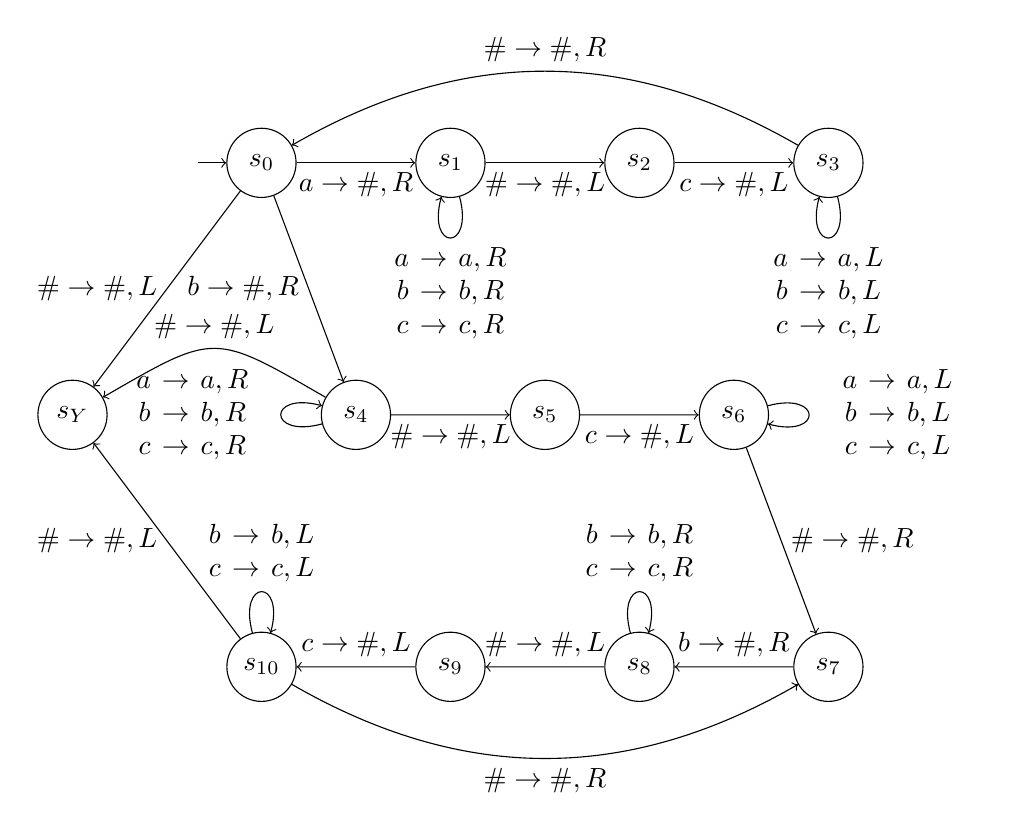
\begin{tikzpicture}[scale=0.8]
        \node[state, initial, initial text=] (s0) at (0, 0) {$s_0$};
        \node[state] (s1) at (3, 0) {$s_1$};
        \node[state] (s2) at (6, 0) {$s_2$};
        \node[state] (s3) at (9, 0) {$s_3$};
        
        \node[state] (sY) at (-3, -4) {$s_Y$};
        
        \node[state] (s4) at (1.5, -4) {$s_4$};
        \node[state] (s5) at (4.5, -4) {$s_5$};
        \node[state] (s6) at (7.5, -4) {$s_6$};
        
        \node[state] (s10) at (0, -8) {$s_{10}$};
        \node[state] (s9) at (3, -8) {$s_9$};
        \node[state] (s8) at (6, -8) {$s_8$};
        \node[state] (s7) at (9, -8) {$s_7$};
        
        \draw[->] (s0) to node[below] {$a \to \#, R$} (s1);
        \draw[->] (s1) to node[below] {$\# \to \#, L$} (s2);
        \draw[->] (s2) to node[below] {$c \to \#, L$} (s3);
        
        \draw[->] (s3) to[bend right, looseness=1] node[above] {$\# \to \#, R$} (s0);
        
        \draw[->] (s1) to[loop below] node[below, text width=2cm, align=center] {$a \to a, R$ $b \to b, R$ $c \to c, R$} (s1);
        \draw[->] (s3) to[loop below] node[below, text width=2cm, align=center] {$a \to a, L$ $b \to b, L$ $c \to c, L$} (s3);
        
        
        \draw[->] (s4) to node[below] {$\# \to \#, L$} (s5);
        \draw[->] (s5) to node[below] {$c \to \#, L$} (s6);
        
        \draw[->] (s4) to[loop left] node[left, text width=2cm, align=center] {$a \to a, R$ $b \to b, R$ $c \to c, R$} (s4);
        \draw[->] (s6) to[loop right] node[right, text width=2cm, align=center] {$a \to a, L$ $b \to b, L$ $c \to c, L$} (s6);


        \draw[->] (s7) to node[above] {$b \to \#, R$} (s8);
        \draw[->] (s8) to node[above] {$\# \to \#, L$} (s9);
        \draw[->] (s9) to node[above] {$c \to \#, L$} (s10);
        
        \draw[->] (s10) to[bend right, looseness=1] node[below] {$\# \to \#, R$} (s7);
        
        \draw[->] (s8) to[loop above] node[above, text width=2cm, align=center] {$b \to b, R$ $c \to c, R$} (s8);
        \draw[->] (s10) to[loop above] node[above, text width=2cm, align=center] {$b \to b, L$ $c \to c, L$} (s10);
        
        
        \draw[->] (s0) to node[left] {$b \to \#, R$} (s4);
        \draw[->] (s6) to node[right] {$\# \to \#, R$} (s7);
        
        \draw[->] (s0) to node[left] {$\# \to \#, L$} (sY);
        \draw[->] (s4) to[bend right, looseness=1.5] node[above] {$\# \to \#, L$} (sY);
        \draw[->] (s10) to node[left] {$\# \to \#, L$} (sY);
    \end{tikzpicture}
    \caption{A Turing machine that recognises strings of the form $a^n b^m c^{n+m}$ for $m, n \geq 0$}
\end{figure}
\noindent Any path not shown is connected to $s_N$.

\subsection{Turing Machines as Functions}
A Turing machine can be thought of as a function. For instance, say that a Turing machine accepts the language $L$. In that case, it can be thought of as computing a function $f$, where $f(x) = 1$ if $x \in L$ and $0$ otherwise.

We can further extend this to use Turing machines to compute a function. It has a set $H$ of halting states, and the function it computes is defined by $f(x) = y$, where $x$ is the initial string on the tape, and $y$ is the string on the tape when the machine halts. For example, the palindrome TM could be redefined so that it deletes the tape contents, and instead of entering $s_Y$, it writes 1 on the tape and enters a halt state, or instead of entering $s_N$, it writes 0 on the tape and enters a halt state.

We will now construct a Turing machine that computes the function $f(k) = k+1$, where the input is in binary. If $k = 100010$, we get $k+1 = 100011$- we just change the 0 into a 1. Now, if $k = 100111$, then $k+1 = 101000$- we change all the 1's at the end to a 0, and change the first 0 we encounter into a 1. We have another case- if $k = 11111$, then $k+1 = 100 000$. So, if we cannot find a rightmost 0, then all the entries are 0. In that case, we replace the first blank before the input with 1, then move right. If it is a 1, we replace it with a 0. If we end up at a blank, we halt.

In general, we start by moving to the end of the string. Then, we move back to the left, until the value at the head is not a 1. We then move to the right, converting all the 1's into 0's

So, the pseudocode for this function is:
\lstinputlisting[language=TM]{src/add1.tm}

Now, we consider the states we require. We need the initial state $s_0$, which moves to the right, seeking the end of the input (the first blank). We need the state $s_1$, looking for the rightmost 0 or blank. We need the state $s_2$ to find the first 0 or blank. We change it to 1 and move right, changing 1s into 0s. Finally, we need a halting state $s_3$.

Next, we consider the transitions. From $s_0$, we enter $s_1$ at the first blank. From $s_1$, we enter $s_2$ if we find a 0 or a blank. From $s_2$, we enter $s_3$ at the first blank.

Therefore, the corresponding Turing machine is therefore the following:
\begin{figure}[H]
    \centering
    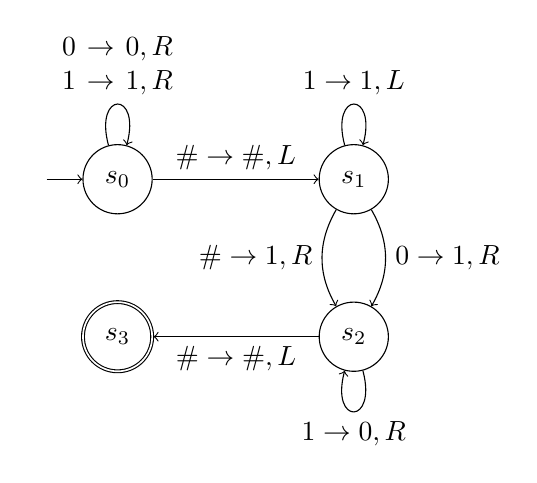
\begin{tikzpicture}
        \node[state, initial, initial text=] (s0) at (0, 0) {$s_0$};
        \node[state] (s1) at (3, 0) {$s_1$};
        \node[state] (s2) at (3, -2) {$s_2$};
        \node[state, accepting] (s3) at (0, -2) {$s_3$};
        
        \draw[->] (s0) to[loop above] node[above, text width=2cm, align=center] {$0 \to 0, R$ $1 \to 1, R$} (s0);
        \draw[->] (s1) to[loop above] node[above] {$1 \to 1, L$} (s1);
        \draw[->] (s0) to node[above] {$\# \to \#, L$} (s1);
        \draw[->] (s1) to[loop above, bend left] node[right] {$0 \to 1, R$} (s2);
        \draw[->] (s1) to[loop above, bend right] node[left] {$\# \to 1, R$} (s2);
        \draw[->] (s2) to node[below] {$\# \to \#, L$} (s3);
        \draw[->] (s2) to[loop below] node[below] {$1 \to 0, R$} (s2);
    \end{tikzpicture}
    \caption{A Turing machine that adds 1 to a binary number.}
\end{figure}

Next, we will construct a Turing machine that returns 1 if it is divisible by 4, and 0 otherwise. The alphabet is $\Sigma = \{0, 1, \#\}$. We will assume that there is at least one non-blank. A binary number is divisible by 4 if the final two digits are 0. The only edge case is 0, which has a single zero. So, a number is divisible by 4 if the last digit is a 0, and the one before it is 0 or blank. In that case, we erase everything and write 1. Otherwise, we erase everything and write 0.

The pseudocode for this function is given below.
\lstinputlisting[language=TM]{src/div4.tm}

So, the Turing machine that checks divisibility by 4 is the following.
\begin{figure}[H]
    \centering
    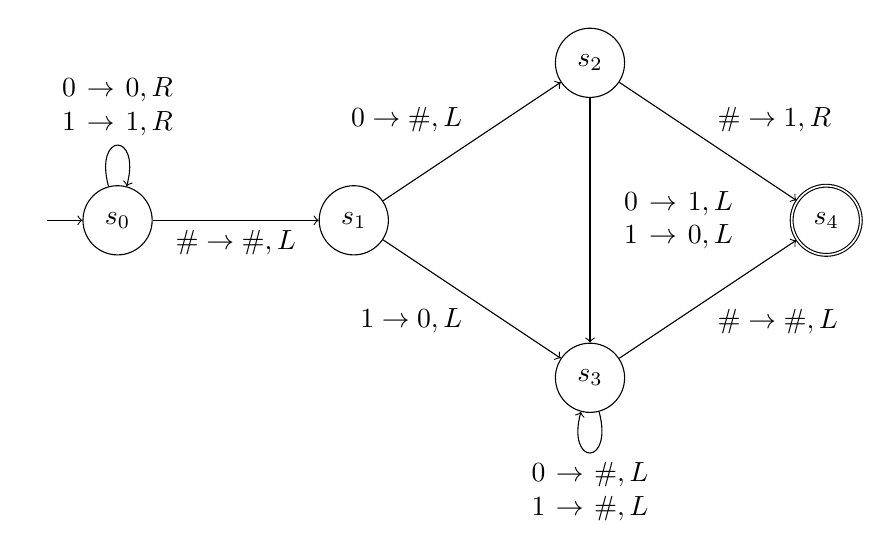
\begin{tikzpicture}
        \node[state, initial, initial text=] (s0) at (0, 0) {$s_0$};
        \node[state] (s1) at (3, 0) {$s_1$};
        \node[state] (s2) at (6, 2) {$s_2$};
        \node[state] (s3) at (6, -2) {$s_3$};
        \node[state, accepting] (s4) at (9, 0) {$s_4$};
        
        \draw[->] (s0) to[loop above] node[above, text width=2cm, align=center] {$0 \to 0, R$ $1 \to 1, R$} (s0);
        \draw[->] (s0) to node[below] {$\# \to \#, L$} (s1);
        \draw[->] (s1) to node[above left] {$0 \to \#, L$} (s2);
        \draw[->] (s1) to node[below left] {$1 \to 0, L$} (s3);
        \draw[->] (s2) to node[above right] {$\# \to 1, R$} (s4);
        \draw[->] (s3) to node[below right] {$\# \to \#, L$} (s4);
        \draw[->] (s2) to node[right, text width=2cm, align=center] {$0 \to 1, L$ $1 \to 0, L$} (s3);
        \draw[->] (s3) to[loop below] node[below, text width=2cm, align=center] {$0 \to \#, L$ $1 \to \#, L$} (s3);
    \end{tikzpicture}
    \caption{A Turing machine that determines whether a binary string is divisible by 4.}
\end{figure}


A language $L$ is Turing-recognisable if there exists some Turing machine that recognises it. That is, given an input string $x$, if $x \in L$, then the TM halts in state $s_Y$. But, if $x \not\in L$, then TM halts in state $s_N$, or it doesn't halt. A language $L$ is Turing-decidable if there exists some Turing machine that decides it. That is, given an input string $x$, if $x \in L$, then the TM halts in state $s_Y$, and if $x \not\in L$, then the TM halts in state $s_N$. 

Clearly, every Turing-decidable language is Turing-recognisable, but not every Turing-recognisable language is Turing-decidable. For example, the language corresponding to the Halting problem is Turing-recognisable, but not decidable. A Turing-recognisable algorithm for the Halting problem would be to run the program on the input, and return true after the program halts. If the program halts, then the execution will stop at some point, and we return true. On the other hand, if the program doesn't halt, the algorithm will not terminate. Therefore, the algorithm is Turing-recognisable, but not decidable.

A function $f: \Sigma^* \to \Sigma^*$ is Turing-computable if there is a Turing machine $M$ such that for any input $x$, the machine $M$ halts with output $f(x)$.

A Turing machine may be enhanced in various ways. For example, we can have multiple tapes, or a 2-dimensional tape. Also, we can make the Turing machine non-deterministic. It turns out that none of these enhancements change the computing power. That is, every language/function that is recognisable/decidable/computable with an enhanced Turing machine is recognisable/decidable/computable with a basic Turing machine. This can be proved by showing that a basic Turing machine can simulate any of these enhanced Turing machines.
\newpage

\section{Counter Programs}
Counter programs are a different model of computation. All general-purpose programming languages have essentially the same computational power. A program written in one language could be translated (or compiled) into a functionally equivalent program in any other. Counter programs are the simplest form of a programming language but with the same computational power.

Counter programs have variables of type \texttt{int}, labelled statements are of the form \texttt{L: unlabelled\_statement}, and unlabelled statements are of the form \texttt{x = 0}, \texttt{x = y+1}, \texttt{x = y-1} or \texttt{if x==0 goto L}, for some labelled statement \texttt{L}, and \texttt{halt}. This has the same computational power as a normal programming language, but is not as easy to code in. For example, we can write a counter program to evaluate the product $x \cdot y$:
\lstinputlisting[language=counter]{src/product.psc}

We have seen that DFA and PDA are not appropriate models of computation. However, it turns out that Turing machines are an appropriate model of computation- this is known as Church-Turing thesis. It is based on the fact that a whole range of different computational models turn out to be equivalent in terms of what they can compute. So, it is reasonable to infer that any one of these models encapsulates what is effectively computable. 

That is, it states that everything `effectively computable' is computable by a Turing machine. It is a thesis and not a theorem since it uses the informal term `effectively computable'. This means that there is an effective procedure for computing the value of the function, including all computers/programming languages that we know about at present, and even those we do not.

There are many equivalent computational models, such as lambda calculus, Turing machines, recursive functions, production systems, counter programs and all general-purpose programming languages. Each of these can simulate the others.


\end{document}
